\chapter{Аналитический раздел}%
\label{cha:analiticheskii_razdel}

% В данном разделе производится анализ предметной области, описываются различные подходы к решению поставленных задач. Также в этом разделе производится формализация задачи и дается описание требуемой функциональности разрабатываемого ПО.

\section{Руткиты}%
\label{sec:rutkity}

Руткит~--- это набор программных инструментов, позволяющих взломать информационную систему. Исторически термин Rootkit пришёл из UNIX, который означал некоторый набор утилит или специальный модуль ядра, который злоумышленник устанавливает на взломанной им компьютерной системе после получения прав суперпользователя. Рутикиты могут включать в себя разный функционал, например предоставление злоумышленнику прав суперпользователя, скрытие файлов и процессов, логирование действий пользователя и другое. Существует множество руткитов, которые реализованы под разные операционные системы. Рутикты могут работать как в пользовательском пространстве, так и в пространстве ядра.

Существует четыре основных вида руткитов:
\begin{itemize}
    \item Руткиты пользовательского уровня;
    \item Руткиты уровня ядра;
    \item Буткиты;
    \item Аппаратные руткиты.
\end{itemize}

\subsection{Руткиты пользовательского уровня} Данные руткиты, которые работают на мои же уровне, что и обычные приложения, установленные и запускаемые пользователем. Чаще всего они перезаписывают функции определенных программ или динамических библиотек, которые загружают пользовательские приложения, чтобы исполнять неавторизованный вредоносный код. Считается, что рутикиты такого вида были одни из первых.

\subsection{Руткиты уровня ядра} Данные руткиты, которые работают как драйверы или загружаемые модули ядра. Программное обеспечение, работающее на этом уровне, имеет прямой доступ к аппаратным и системным ресурсам. Руткиты этого уровня перезаписывают системные вызовы, что затрудняет их обнаружение.

\subsection{Буткиты} Это руткиты, которые записывают свой исполняемый код в основной загрузочный сектор жесткого диска. Благодаря этому они могут получить контроль над устройством ещё до запуска операционной системы. Являются разновидностью руткита уровня ядра.

\subsection{Аппаратные руткиты} Это программное обеспечение, которое скрыто внутри архитектуры компьютера, например в сетевой карте, жёстком диске или в системном BIOS.

\begin{figure}[H]
    \centering
    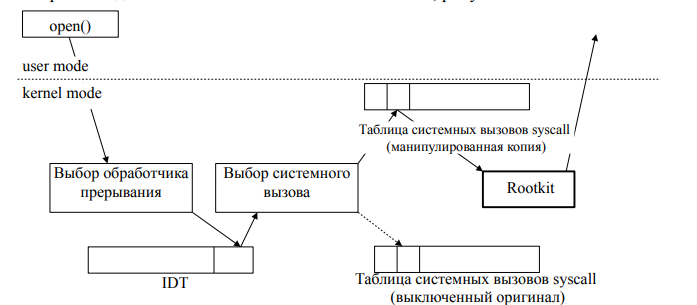
\includegraphics[scale=0.65]{img/rootkit.jpg}
    \caption{Cхема работы руткита}\label{img:rootkit}
\end{figure}

\section{Загружаемый модуль ядра}%
\label{sec:zagruzhaemyi_modul_iadra}

Загружаемый модуль ядра~--- объектный файл, содержащий код, расширяющий возможности ядра операционной системы. Модули используются, чтобы добавить поддержку нового оборудования или файловых систем или для добавления новых системных вызовов. Когда функциональность, предоставляемая модулем, больше не требуется, он может быть выгружен, чтобы освободить память и другие ресурсы.

Основное преимущество и основная причина использования загружаемых модулей ядра заключается в том, что они могут расширять функциональные возможности ядра без необходимости перекомпилировать ядро или даже перезапускать систему. В системах Linux все модули обычно хранятся в каталоге /lib/modules и имеют расширение .ko. Модули загружаются и выгружаются службой modprobe. Основные команды для управления модулями: insmod (загрузка модулей), rmmod (удаление модулей) и lsmod.

Каждый загружаемый модуль ядра должен содержать в себе две ключевые функции: module\_init и module\_exit. Функция module\_init отвечает за выделение дополнительной памяти, необходимой для работы модуля (память для самого модуля выделяется ядром в пространстве памяти ядра), вызывая дополнительные потоки или процессы. Точно так же функция module\_exit отвечает за освобождение ранее выделенной памяти, остановку потоков или процессов и другие операции, необходимые для удаления модуля.

\section{Системные вызовы}%
\label{sec:sistemnye_vyzovy}

В программировании и вычислительной технике системный вызов является программным способом обращения компьютерной программы за определенной операцией от ядра операционной системы. Иными словами, системный вызов возникает, когда пользовательский процесс требует некоторой службы реализуемой ядром и вызывает специальную функцию.

Сюда могут входить услуги, связанные с аппаратным обеспечением (например, доступ к жесткому диску), создание и выполнение новых процессов, связь с интегральными службами ядра, такими как планирование процессов. Системные вызовы обеспечивают необходимый интерфейс между процессом и операционной системой.

Во всех реализациях Linux имеется строго определенное число точек входа в ядро, которые называются системными вызовами.

\subsection{Системные вызовы и библиотечные функции}%
\label{sub:promezhutochnaia_biblioteka}

В системе Linux для каждого системного вызова предусматривается одноименная функция в стандартной библиотеке языка C. Пользовательский процесс вызывает эту функцию как обычно, а она вызывает соответствующую службу ядра,
применяя способ обращения, принятый в данной системе. Например, функция
может поместить один или более своих аргументов в регистры общего назначения и затем выполнить некоторую машинную инструкцию, которая сгенерирует
программное прерывание.

%\begin{figure}[H]
%    \centering
%    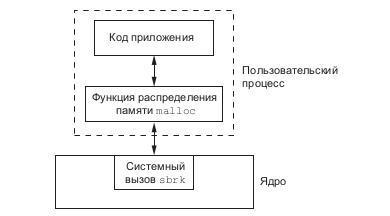
\includegraphics[scale=0.65]{img/sys_call.jpg}
%    \caption{Разделение обязанностей функции malloc и системного вызова sbrk}\label{img:sys_call}
%\end{figure}

\section{Таблица системных вызовов}%
\label{sec:tablitsa_sistemnykh_vyzovov}

Таблица системных вызовов~--- это структура, которая хранит адреса исполняемого кода отдельных системных вызовов в области памяти ядра. По номеру системного вызова в таблица можно определить его адрес в памяти и вызвать его. Начиная с 2.6.x версии ядра linux, адрес таблица системных вызовов не экспортируется в syscalls.h, это сделано для затруднения доступа и редактирования таблицы системных вызовов.

Руткиты используют различные методы для получения адреса таблицы системных вызовов, чтобы иметь возможность редактировать или заменять ее.

\section{Анализ способов перехвата функций в ядре}%
\label{sec:analiz_sposobov_perekhvata_funktsii_v_iadre}

В рамках данного проекта необходимо осуществить перехват некоторых функций, то есть получение управления функции в момент её вызова.

Сегодня существует множество подходов для перехвата функций в ядре. 

Рассмотрим самые распространенные из них:

\subsection{Модификация таблицы системных вызовов}%
\label{sub:modifikatsiia_tablitsy_sistemnykh_vyzovov}

Как известно, Linux хранит все обработчики системных вызовов в таблице sys\_call\_table. Подмена значений в этой таблице приводит к смене поведения всей системы. Таким образом, сохранив старое значения обработчика и подставив в таблицу собственный обработчик, мы можем перехватить любой системный вызов.

Алгоритм перехвата системных вызовов с помощью модификации таблицы системных вызовов следующий:
\begin{itemize}
    \item
        сохранить указатель на оригинальный (исходный) вызов для возможности его восстановления;
    \item
    создать функцию, реализующую новый системный вызов;
    \item
    в таблице системных вызовов sys\_call\_table произвести замену вызовов, т.е. настроить соответствующий указатель на новый системный вызов;
    \item
    по окончании работы (при выгрузке модуля) восстановить оригинальный системный вызов, используя ранее сохраненный указатель.
    \item 
    можно перехватить только системные вызовы – нельзя перехватить
	обычные функции.
\end{itemize}

\subsection{Kernel tracepoints}%


Kernel tracepoints~--- это фреймворк для трассировки ядра, реализованный через статическое инструментирование кода. Большинство
важных функций ядра статически инструментировано – в теле функций
добавлены вызовы функций фреймворка рассматриваемого фреймворка.

Особенности рассматриваемого фреймворка:

\begin{itemize}
	\item минимальные накладные расходы – необходимо только вызвать функцию трассировки в необходимом месте;
	\item отсутствие задокументированного интерфейс;
	\item не все функции ядра статически инструментированны;
	\item не работает, если ядро не сконфигурировано должным образом.
\end{itemize}

\subsection{Kprobes}%
\label{sub:kprobes}

Kprobes~--- специальный интерфейс, предназначенный для отладки
и трассировки ядра. Данный интерфейс позволяет устанавливать пред и
пост-обработчики для любой инструкции в ядре, а так же обработчики на
вход и возврат из функции. Обработчики получают доступ к регистрам и
могут изменять их значение. Таким образом, kprobes можно использовать
как и в целях мониторинга, так и для возможности повлиять на дальнейший ход работы ядра.

Особенности рассматриваемого интерфейса:

\begin{itemize}
	\item перехват любой инструкции в ядре – это реализуется с помощью точек останова (инструкция int3), внедряемых в исполняемый код ядра. Таким образом, можно перехватить любую функцию в ядре;
	\item хорошо задокументированный интерфейс;
	\item нетривиальные накладные расходы – для расстановки и обработки
		точек останова необходимо большое количество процессорного времени;
	\item техническая сложность реализации. Так, например, чтобы получить
		аргументы функции или значения её локальных переменных нужно
		знать, в каких регистрах, или в каком месте на стеке они находятся,
		и самостоятельно их оттуда извлекать;
	\item при подмене адреса возврата из функции используется стек, реализо-
		ванный с помощью буффера фиксированного размера. Таким обра-
		зом, при большом количестве одновременных вызовов перехваченной
		функции, могут быть пропущены срабатывания.
\end{itemize}

\subsection{ftrace}

ftrace - это фреймворк для трассировки ядра на уровне функций, реализованный на основе ключей компилятора -pg и mfentry.
Данные функции вставляют в начало каждой функции вызов специальной
трассировочной функции mcount() или \_\_fentry()\_\_. В пользовательских
программах данная возможность компилятора используется профилировщиками, с целью отслеживания всех вызываемых функций. В ядре эти
функции используются исключительно для реализации рассматриваемого
фреймворка.

Для большинства современных архитектур процессора доступна опти-
мизация: динамический frace.
Ядро знает расположение всех вызовов функций mcount() или \_\_fentry()\_\_ и на ранних этапах загрузки ядра
подменяет их машинный код на специальную машинную инструкцию NOP, которая ничего не делает. При включении трассировки, в нужные функ-
ции необходимые вызовы добавляются обратно. Если ftrace не использу-
ется, его влияние на производительность системы минимально.

Особенности рассматриваемого фреймворка:

\begin{itemize}
	\item имеется возможность перехватить любую функцию;
	\item перехват совместим с трассировкой;
	\item фреймворк зависит от конфигурации ядра, но, в популярных конфигурациях ядра (и, соответственно, в популярных образах ядра)
		установлены все необходимые флаги для работы;
\end{itemize}

\subsection*{Сравнение методов}

В таблице \ref{tab:analyze} приведено сравнение приведенных выше методов, позволяющих перехватывать системные вызовы.

\begin{table}[H]
	\centering
	\begin{tabular}{ | p{3cm} | p{2cm} | p{2cm} | p{2cm} | }
		\hline
		Название & Дин. загрузка & Перехват любых функций & Любая конфигурация ядра \\
		\hline
		Модификация таблицы системных вызовов & Да & Нет & Да \\
		\hline
		kprobes & Да & Да & Да\\
		\hline
		kernel tracepoints & Да & Да & Нет \\
		\hline
		ftrace & Да & Да & Нет \\
		\hline
	\end{tabular}
	\caption{\label{tab:analyze} Методы перехвата системных вызовов}
\end{table}

\section{Диагностика процессов}%
\label{sec:diagnostika_protsessov}

Для изучения операционной системы linux и используемых программ могут понадобиться средства диагностики процессов. В операционной системе linux есть утилиты, которые позволяют наблюдать системные вызовы, которые использует программа. Изучая системные вызовы, которые использует программа, можно узнать, к каким файлам обращается программа, какие сетевые порты она использует, какие ресурсы ей нужны, а также какие ошибки возвращает ей система.

Одной из таких утилит является strace. С помощью strace можно узнать, какие системные вызовы исполняет программа, а также их параметры и результат их выполнения.

В самом простом варианте strace запускает переданную команду с её аргументами и выводит в стандартный поток ошибок все системные вызовы команды.


\section*{Выводы}%
\label{sec:vyvody}

В рамках данного проекта было принято решение использовать загружаемый модуль ядра для реализации руткита. Данный подход обеспечивает наименьшую вероятность обнаружения антивирусными программами. Также данный подход позволяет расширять функциональность руткита без необходимости перекомпилировать ядро.

Для подмены системных вызовов было принято решение использовать фреймворк ftrace. Такое решение предоставляет возможность перехватывать не только системные вызовы, но и другие функции ядра, что может быть полезно.

Преимущество этого решения состоит в том, что таблица системных вызовов никоим образом не изменяется. Программы, используемые для обнаружения руткитов в системе очень часто сравнивают содержимое таблицы системных вызовов в памяти с содержимым, хранящимся в каталоге /boot. В случае использования выбранного решения они не обнаружат никаких различий и не вызовут тревогу.
